\section{Background Information \& Research}
This sections look at some software systems that are already attempting to solve the problem identified in this dissertation, as well as discussing some of the different technologies considered for the implementation of this project.

\subsection{Existing Systems}
\label{sec:existing-systems}
As mentioned in section \ref{sec:intro}, software systems for the distribution and sharing of scenic routes already exist. Each of these systems approaches the problem in a different way, and thus all have their own advantages and disadvantages, which will be discussed here. The aim of this is to determine the best features and the worst features, so they can be incorporate or avoided.

\paragraph{Google's ``My Maps'', \url{https://www.google.com/maps/d}}\ \\
Google's ``My Maps'' service (distinct from ``Google Maps'') is a tool that offers users the ability to plot maps between locations, and save them to their Google accounts. This allows users to quickly access routes they travel frequently, as well share those routes with others (over various social media platforms). The main advantages of this service are that it provides a graphical tool for visualising routes, the ability to add photos and videos to specific waypoints, and, as mentioned above, the ability to share routes via social media. Another interesting feature that is provided is the ability to plot all the point, and generate the route afterwards, rather than generating the route after each point is placed. This is an interesting consideration for a mobile application, because users may wish to save on data (although if users are unaware of this being the reason, it just makes the tool look less responsive).\ \\
\ \\
The key disadvantage of Google's ``My Maps'' is that it is very slow, and there are long periods of loading in-between successive actions. Responsiveness on websites is key, otherwise users are unaware if their actions are having an impact or not. There are also other disadvantages, including the unintuitive and cluttered user interface, the small user base (being a relatively unknown piece of software, dwarfed by the Google Maps service), and that the only way of sharing your routes is to other social media platforms. This last point is particularly important to address for Niceway.to, because it aims is to build a community of users. If they can only share their routes to \textit{other} platforms, the community will have a much smaller chance of thriving. This is why all routes on Niceway.to will be accessible and searchable from within the system itself, and the sharing of routes will simply be a tool to draw more people to the site.

\begin{figure}[!ht]
	\begin{center}
		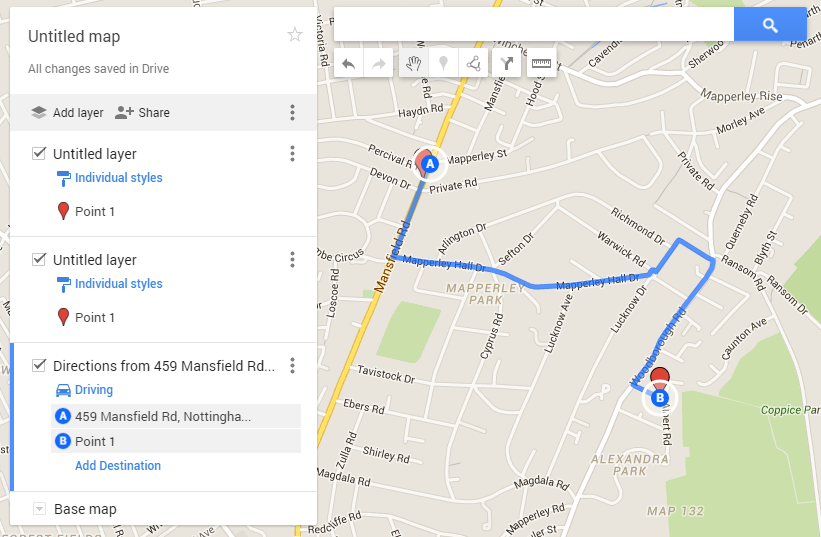
\includegraphics[width=0.66\textwidth]{images/background/gm_rcp.png}
	\end{center}
	\vspace{-6mm}
	\caption{Google's ``My Maps'' route creation/editing feature}
	\vspace{-6mm}
\end{figure}

\newpage 
\paragraph{MyScenicDrives, \url{https://www.myscenicdrives.com}}
\begin{wrapfigure}{r}{0.45\textwidth}
	\vspace{1mm}
	\begin{center}
		\hspace{5mm}
		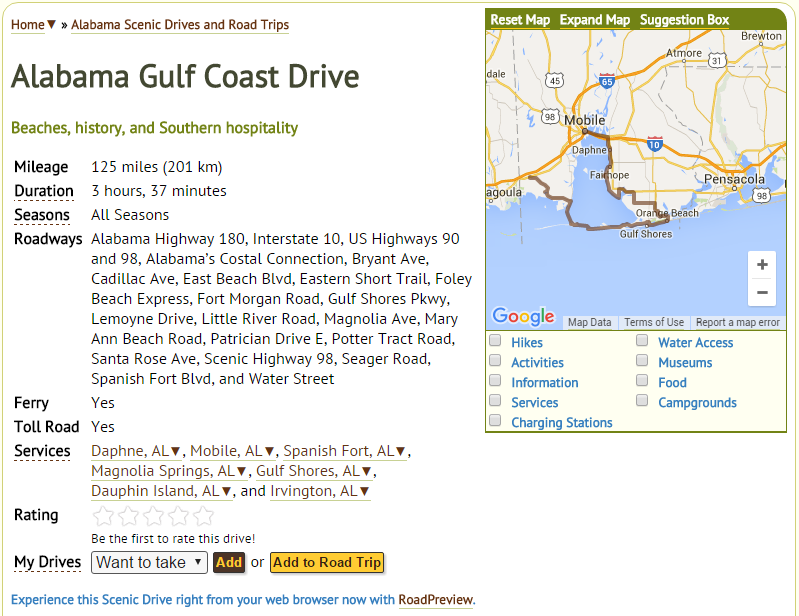
\includegraphics[width=0.45\textwidth]{images/background/msd_rdp.png}
	\end{center}
	\vspace{-6mm}
	\caption{MyScenicDrive's route details}	
	\vspace{-10mm}
\end{wrapfigure}
MyScenicDrives is a website that allows users to search for scenic routes by city, state or zip code (currently the service is only available in the United States), and view extremely detailed information about these routes. This includes a very lengthy explanation of all the things can be seen and done on the journey, interesting facts about the locations visited, all the roads that will be driven on, the best seasons to take the journey during, and even which service stations will be passed. This extremely rich content is the main selling of MyScenicDrives.

\vspace{5mm}
\noindent 
However, no matter how high the quality of this content it, there is still a glaring problem with MyScenicDrives: the quantity of routes. This may be due to the huge amount of information required for a route to be accepted onto the site, but essentially makes the entire application useless. As an example, a search for all routes in the state of Alabama returned a single result. In addition to this, the search functionality itself is very primitive. There is no option for users to select where they wish to start or end their journey, and instead they can only pick a large geographic region. Which would not be suitable for Niceway.to, which aims to provide a way for users to find routes between specific locations.
\ \\
\paragraph{Mad Maps, \url{http://madmaps.net/}}\ \\
The final mapping website that was investigated was Mad Maps, which differed from the others in that it allowed users to purchase physical maps, which they could also view on their mobile phones. One useful feature of the service was the ability to download routes directly to a mobile device, so that the user's Internet connection did not become a limiting factor during a journey. However, it is difficult to ignore the biggest down fall of this service, which was the cost associated with it. All of the maps had a price associated with them, and there was no ability to preview the maps before purchasing. This blind investment could be off putting for many users, as they may be unsure if they will even enjoy the routes provided. Further to this, the mobile application both required an upfront payment to download, as well as containing adverts within it: which seems unjustified when the majority of the Mad Maps applications had very poor reviews.
\begin{wrapfigure}{l}{0.4\textwidth}
	\vspace{-1mm}
	\hspace{5mm}
	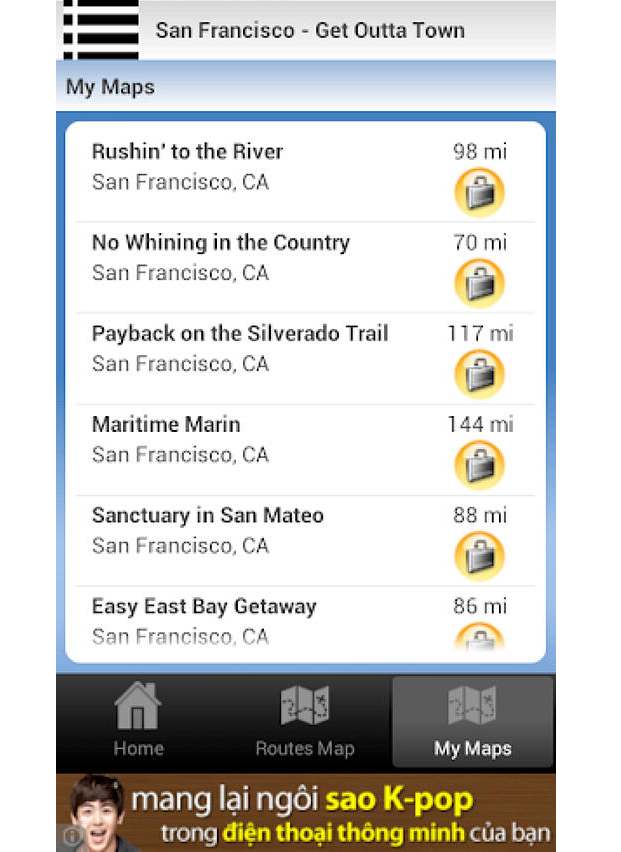
\includegraphics[width=0.35\textwidth]{images/background/mm_rlp.png}
	\centering
	\caption{List of Mad Maps routes}	
	\vspace{-40mm}
\end{wrapfigure}
\ \\
The service works by having a group of ``experts'' compile the maps, and distribute them to the users. This is supposed to instil confidence of their quality, but instead takes out a huge part of travelling, which is the social experience. The only social interaction that users can have with Mad Maps, is the ability to upload photos of waypoints that they have visited, but these will then only be seen by other users that have purchased the route, and would not help to foster the community that Niceway.to is striving for. 

\newpage 
\subsection{Platforms and Tools}
\label{sec:pat}
This section introduces some potential platforms and tools that could have been used in the project, along with justifications for and against them. The system consisted of the back end and server technologies, as well as some user-friendly front end. Tools and frameworks and languages for both of these parts were evaluated to determine which would be the most appropriate. A full list of the final decisions of tools to use, including their justifications, can be found in section \ref{sec:kid}.

\subsubsection{Native Mobile Applications VS Responsive Web Applications}
Before investigating technologies to use, it was important to determine what kind of application was to be developed, as this would radically change the tools required. Ultimately, it was decided that it would be better to build Niceway.to as a responsive web-application, but the advantages and disadvantages of both approaches have been discussed below.

\paragraph{Native Mobile Application}\ \\
Native mobile applications are applications that are downloaded onto a mobile device, and run directly on the hardware. These applications generally have greater exposure, because they are distributed through the application marketplace for the given operating system, and can be reviewed and rated by users. There are several advantages to developing a native mobile application including: the ability to implement multiple pricing models (payment for download, in-application purchases, free with advertisements, or entirely free), after the initial download they can be used without an Internet connection (as data can be downloaded to the phone and accessed later), and the native technology and hardware of the phone can be utilised to provide a better experience for the user.\ \\
\ \\
However, native applications do also have some drawbacks. The most prominent is the number of different operating systems available, which mean that any application created needs to be rewritten multiple times in different languages, to ensure that it can target all devices. This is a huge investment of time and resources, especially as some platforms do not have a large user base (and therefore this effort would potentially be wasted). Native applications must also be downloaded onto the user's device, which requires a commitment from the user, and their on-going desire to keep the application on their phone. Mobile phone users can be fickle, and delete the application at any time for any number of reasons. 

\paragraph{Responsive Web Application}\ \\
A responsive web application is a website that can function both on desktop devices, and mobile devices by scaling the elements on display. They are incredibly versatile because they run in a web browser, which means that they target all possible devices without the need to rewrite the code base in several languages (some tweaks for certain browsers may be required, but this is usually a small amount of work). They are written in the default web languages of HTML, CSS and JavaScript, and the back end can be whichever language the developers are most comfortable with, which makes it very easy for developers of any skill level to work on them. Another advantage of them being hosted on a server online is that it becomes very easy to release updates, because they are instantaneous, and the users do not have to download anything.\\
\ \\
However, the Internet is a large place, and without a centralised place to advertise the application, it is possible it will never be discovered by many potential users. Alongside this, web applications require a constant Internet connection to access them, which could be a problem for users that do not have a large data allowance on their phone.


\newpage 
\subsubsection{Back End Tools}
{\color{purple}
Language  - framework pairs
}

\paragraph{The Zend Framework (PHP)}\ \\
{\color{red} What is it, why it's good, why it's not}

\paragraph{Ruby on Rails?}\ \\
{\color{red} What is it, why it's good, why it's not}

\paragraph{Javascript with Node.js}\ \\
{\color{red} What is it, why it's good, why it's not - good because all one language!}


\subsubsection{Front End Tools}
{\color{purple}
After it was decided that it was to be a web app, the language choice was obvious, so I looked at front-end design frameowkrs instead instead.
}
\paragraph{Bootstrap}\ \\
{\color{red} What is it, why it's good, why it's not}

\paragraph{Foundation}\ \\
{\color{red} What is it, why it's good, why it's not}

\paragraph{Semantic}\ \\
{\color{red} What is it, why it's good, why it's not}